% =====================================================================
%  Campus Event Management Platform: presentation slides (5 minutes)
%  Build:  ./scripts/build_docs.sh      (or upload report/ to Overleaf)
% =====================================================================
\documentclass[aspectratio=169,11pt]{beamer}
\usetheme{Madrid}
\usecolortheme{default}
\setbeamertemplate{navigation symbols}{}          % hide the little navigation icons
\setbeamertemplate{itemize items}[circle]

\usepackage[T1]{fontenc}
\usepackage[utf8]{inputenc}
\usepackage{booktabs}
\usepackage{listings}
\usepackage{tikz}
\usetikzlibrary{positioning,arrows.meta,fit,shapes.geometric}
\usepackage{pgfplots}
\pgfplotsset{compat=1.17}

\newcommand{\code}[1]{\texttt{\detokenize{#1}}}

\lstset{basicstyle=\ttfamily\scriptsize, breaklines=true, columns=fullflexible,
        keepspaces=true, showstringspaces=false, frame=single, rulecolor=\color{black!20},
        backgroundcolor=\color{black!3}, keywordstyle=\color{blue!70!black}\bfseries,
        commentstyle=\color{green!40!black}\itshape}

\title[Campus Event Management Platform]{Campus Event Management Platform}
\subtitle{Flask + SQLite, tested and profiled}
\author{Prajyot MC25BT012}
\institute[CS 202C]{CS 202C}
\date{November 2026}

\begin{document}

% ---------------------------------------------------------------------
% 1
\begin{frame}
  \titlepage
\end{frame}

% ---------------------------------------------------------------------
% 2
\begin{frame}{The problem and the course modules}
  \begin{columns}[T]
    \begin{column}{0.47\textwidth}
      \textbf{Problem}
      \begin{itemize}
        \item Campus events are announced on posters and in chat groups
        \item Sign-ups are tracked in spreadsheets: no limit on seats
        \item Two events can be booked into the same hall at the same time
        \item No overview of which events and venues are popular
      \end{itemize}
      \vspace{4pt}
      \textbf{Goal:} one simple web app for students and admins, built so I can explain every line.
    \end{column}
    \begin{column}{0.5\textwidth}
      \small
      \begin{tabular}{@{}l l@{}}
        \toprule
        \textbf{Module} & \textbf{Used for} \\
        \midrule
        HTML/CSS & Jinja2 templates, hand-written CSS \\
        Python   & Flask, Blueprints, pytest, cProfile \\
        SQL      & raw \code{sqlite3}, JOINs, indexes \\
        Git      & 23+ small conventional commits \\
        Bash     & setup/run/seed/test/profile scripts \\
        LaTeX    & this deck + the report \\
        \bottomrule
      \end{tabular}
    \end{column}
  \end{columns}
\end{frame}

% ---------------------------------------------------------------------
% 3
\begin{frame}{Architecture}
  \centering
  \resizebox{0.95\textwidth}{!}{%
  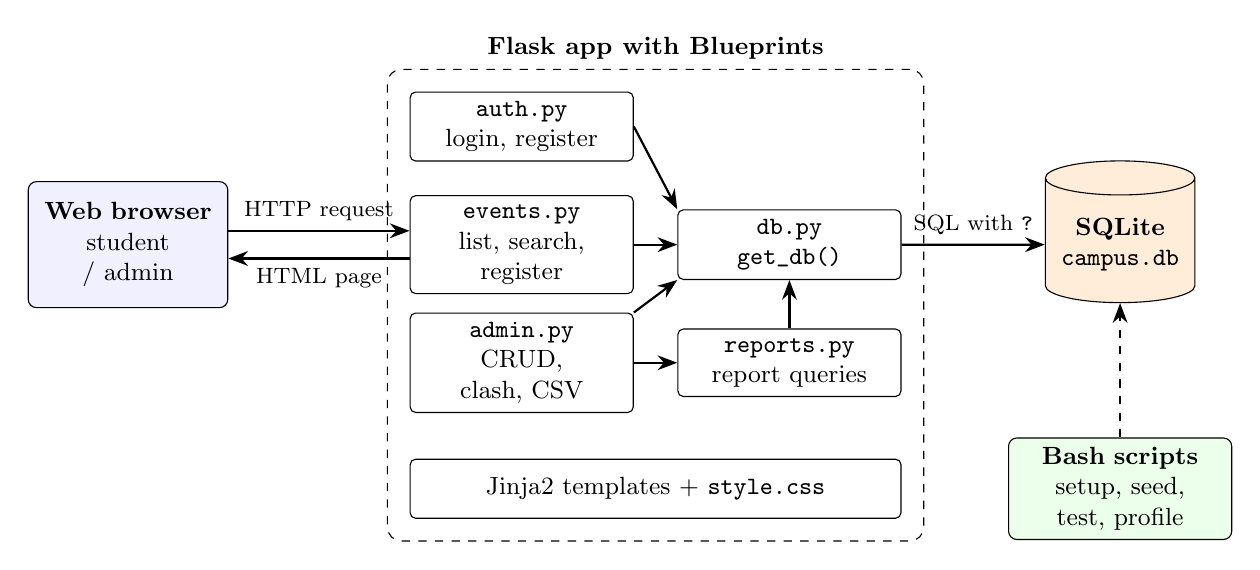
\begin{tikzpicture}[
      font=\small,
      box/.style={draw, rounded corners=3pt, fill=blue!6, align=center, minimum height=0.9cm, text width=2.5cm},
      mod/.style={draw, rounded corners=2pt, fill=white, align=center, minimum height=0.75cm, text width=2.6cm},
      arr/.style={-{Stealth[length=2.5mm]}, thick},
    ]
    \node[box, text width=2.3cm, minimum height=1.6cm] (browser) at (0,0) {\textbf{Web browser}\\ student / admin};
    \node[mod] (auth)    at (5,1.5)    {\code{auth.py}\\ login, register};
    \node[mod] (events)  at (5,0)      {\code{events.py}\\ list, search, register};
    \node[mod] (admin)   at (5,-1.5)   {\code{admin.py}\\ CRUD, clash, CSV};
    \node[mod] (reports) at (8.4,-1.5) {\code{reports.py}\\ report queries};
    \node[mod] (db)      at (8.4,0)    {\code{db.py}\\ \code{get_db()}};
    \node[mod, text width=6cm] (tpl) at (6.7,-3.1) {Jinja2 templates + \code{style.css}};
    \node[draw, dashed, rounded corners=5pt, inner sep=8pt, fit=(auth)(admin)(reports)(db)(tpl),
          label={[font=\small\bfseries]above:Flask app with Blueprints}] (flask) {};
    \node[draw, shape=cylinder, shape border rotate=90, aspect=0.25, fill=orange!15,
          minimum height=1.8cm, minimum width=1.9cm, align=center] (sqlite) at (12.6,0)
          {\textbf{SQLite}\\ \code{campus.db}};
    \node[box, fill=green!8, text width=2.6cm] (bash) at (12.6,-3.1)
          {\textbf{Bash scripts}\\ setup, seed, test, profile};
    \draw[arr] ([yshift=5pt]browser.east) -- node[above, font=\footnotesize]{HTTP request} ([yshift=5pt]events.west);
    \draw[arr] ([yshift=-5pt]events.west) -- node[below, font=\footnotesize]{HTML page} ([yshift=-5pt]browser.east);
    \draw[arr] (auth.east)   -- (db.north west);
    \draw[arr] (events.east) -- (db.west);
    \draw[arr] (admin.east)  -- (reports.west);
    \draw[arr] (admin.north east) -- (db.south west);
    \draw[arr] (reports.north) -- (db.south);
    \draw[arr] (db.east) -- node[above, font=\footnotesize]{SQL with \code{?}} (sqlite.west);
    \draw[arr, dashed] (bash.north) -- (sqlite.south);
  \end{tikzpicture}}

  \vspace{6pt}
  \small App factory \code{create_app()} $\cdot$ one DB connection per request $\cdot$
  every SQL value through a \code{?} placeholder $\cdot$ passwords stored as salted hashes
\end{frame}

% ---------------------------------------------------------------------
% 4
\begin{frame}{Database schema}
  \begin{columns}[c]
    \begin{column}{0.55\textwidth}
      \centering
      \resizebox{\textwidth}{!}{%
      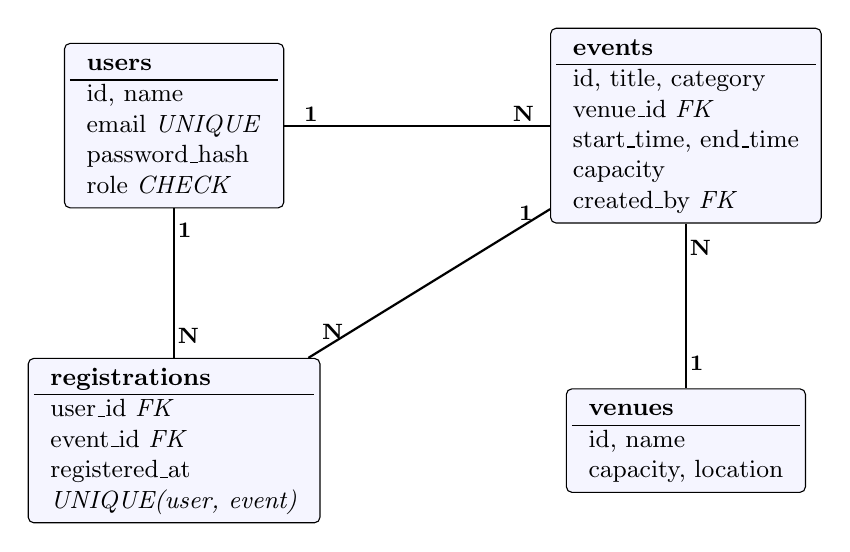
\begin{tikzpicture}[
          entity/.style={draw, rounded corners=2pt, fill=blue!4, font=\small, inner sep=2pt},
          rel/.style={draw, thick},
          card/.style={font=\footnotesize\bfseries, inner sep=1pt},
        ]
        \node[entity] (users) at (0,0) {\begin{tabular}{l}\textbf{users}\\ \hline
          id, name\\ email \textit{UNIQUE}\\ password\_hash\\ role \textit{CHECK}\end{tabular}};
        \node[entity] (events) at (6.5,0) {\begin{tabular}{l}\textbf{events}\\ \hline
          id, title, category\\ venue\_id \textit{FK}\\ start\_time, end\_time\\ capacity\\ created\_by \textit{FK}\end{tabular}};
        \node[entity] (regs) at (0,-4) {\begin{tabular}{l}\textbf{registrations}\\ \hline
          user\_id \textit{FK}\\ event\_id \textit{FK}\\ registered\_at\\ \textit{UNIQUE(user, event)}\end{tabular}};
        \node[entity] (venues) at (6.5,-4) {\begin{tabular}{l}\textbf{venues}\\ \hline
          id, name\\ capacity, location\end{tabular}};
        \draw[rel] (users) -- node[card, pos=0.1, above]{1} node[card, pos=0.9, above]{N} (events);
        \draw[rel] (users) -- node[card, pos=0.15, right]{1} node[card, pos=0.85, right]{N} (regs);
        \draw[rel] (regs)  -- node[card, pos=0.1, above]{N} node[card, pos=0.9, above]{1} (events);
        \draw[rel] (events) -- node[card, pos=0.15, right]{N} node[card, pos=0.85, right]{1} (venues);
      \end{tikzpicture}}
    \end{column}
    \begin{column}{0.42\textwidth}
      \small
      \begin{itemize}
        \item The database enforces the rules itself:\\
              \code{UNIQUE}, \code{CHECK (end_time > start_time)}, foreign keys
        \item \code{UNIQUE(user_id, event_id)}: no double registration, even with a bug
        \item \code{ON DELETE CASCADE}: deleting an event removes its registrations
        \item Times stored as \code{'YYYY-MM-DD HH:MM'}, so text order = time order
      \end{itemize}
    \end{column}
  \end{columns}
\end{frame}

% ---------------------------------------------------------------------
% 5
\begin{frame}{Features}
  \begin{columns}[T]
    \begin{column}{0.48\textwidth}
      \textbf{Students}
      \begin{itemize}\small
        \item Register / log in (hashed passwords)
        \item Search by keyword, category, venue, dates
        \item Register; refused if \emph{full}, \emph{started} or \emph{already registered}
        \item Cancel, ``My registrations''
      \end{itemize}
      \textbf{Admins}
      \begin{itemize}\small
        \item CRUD for events and venues
        \item \textbf{Venue clash check}:\\ \code{start < other_end AND end > other_start}
        \item Participants + CSV export
        \item Reports: fill rate, categories, venues
      \end{itemize}
    \end{column}
    \begin{column}{0.5\textwidth}
      \centering
      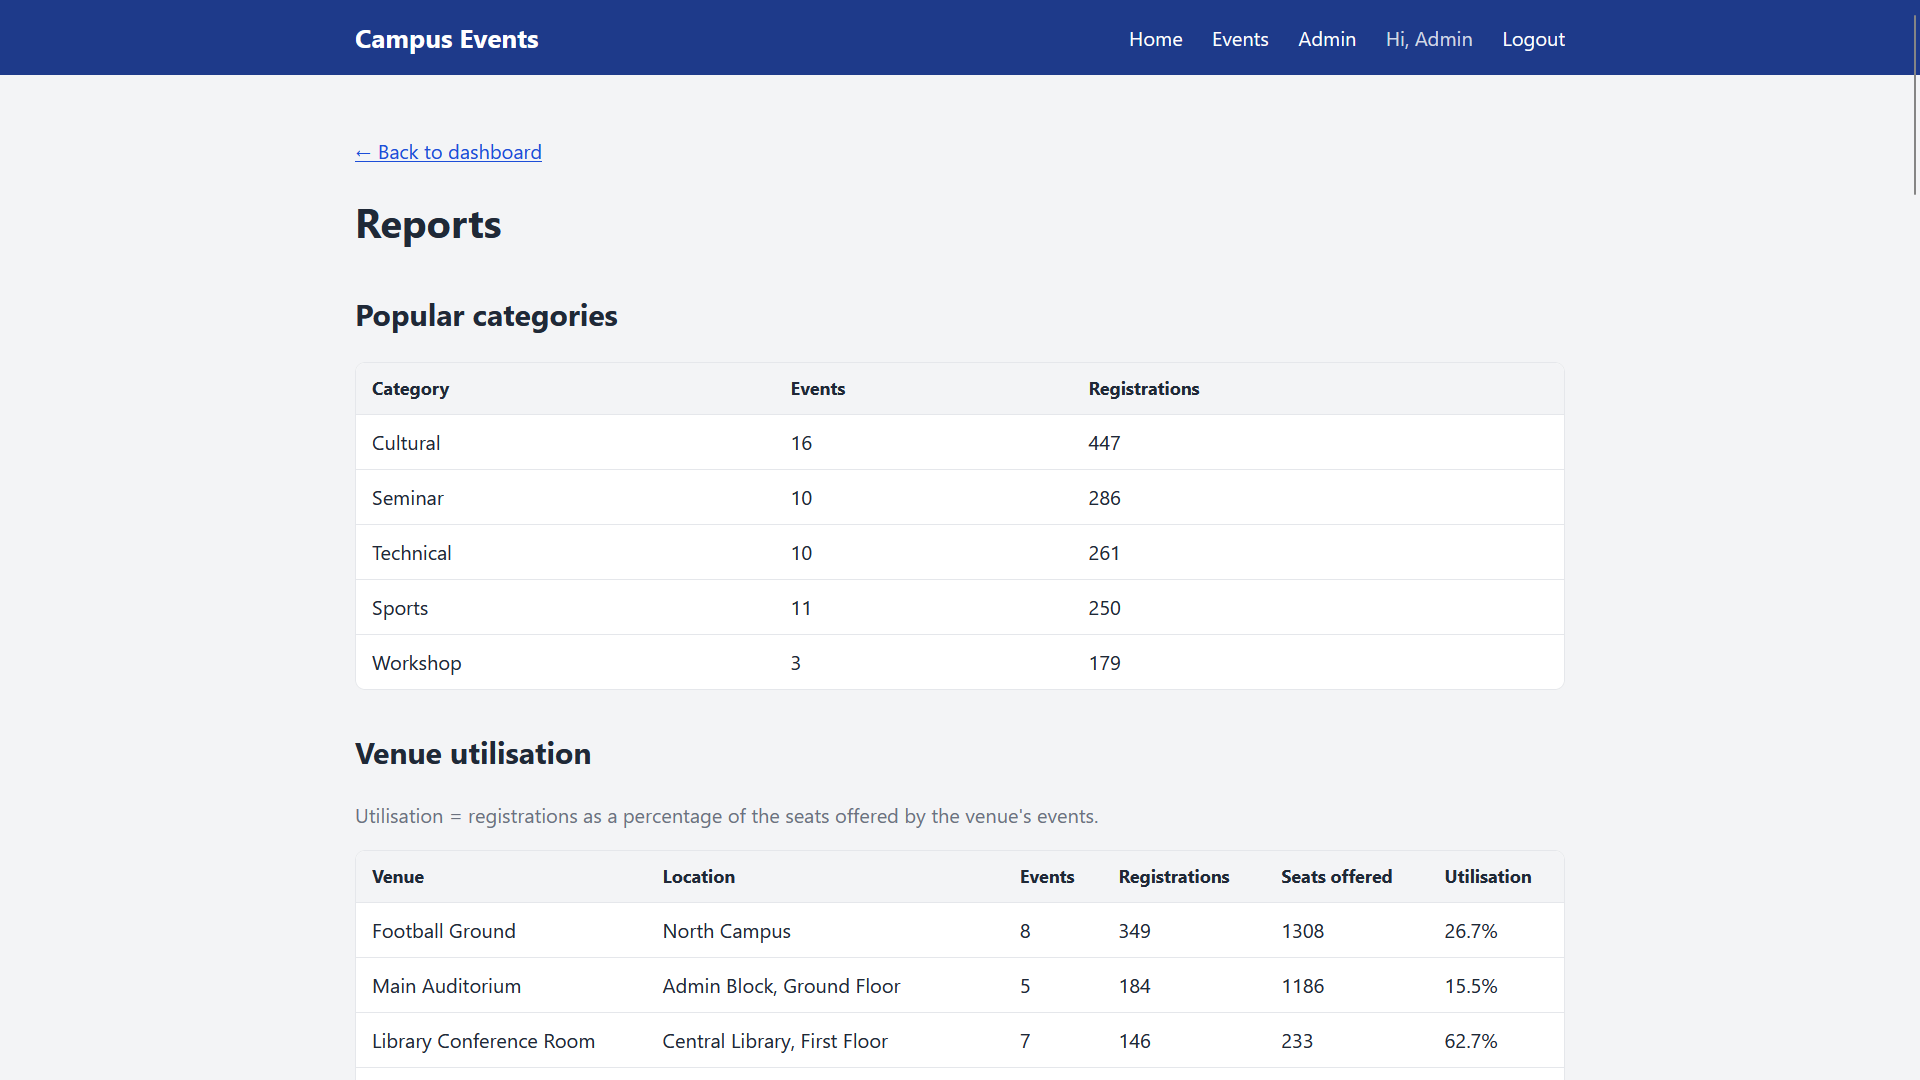
\includegraphics[width=\textwidth]{figures/reports_overview.png}\\[2pt]
      {\scriptsize Reports page (demo data)}
    \end{column}
  \end{columns}
\end{frame}

% ---------------------------------------------------------------------
% 6
\begin{frame}{Testing: 45 pytest tests, all passing}
  \begin{columns}[c]
    \begin{column}{0.5\textwidth}
      \small
      \begin{tabular}{@{}l r@{}}
        \toprule
        \textbf{Area} & \textbf{Tests} \\
        \midrule
        Authentication and roles & 7 \\
        Browsing and search      & 5 \\
        Registrations            & 8 \\
        Admin CRUD, clashes, CSV & 18 \\
        Reports                  & 7 \\
        \midrule
        \textbf{Total}           & \textbf{45} \\
        \bottomrule
      \end{tabular}
    \end{column}
    \begin{column}{0.47\textwidth}
      \small
      \begin{itemize}
        \item Each test gets a \textbf{fresh temporary database}
        \item \code{find_clash()} tested on its own: overlap, touching, other venue, ignore itself
        \item Report tests check \textbf{exact numbers}, so they prove the optimised version gives the same answers
        \item Run with \code{./scripts/test.sh}
      \end{itemize}
    \end{column}
  \end{columns}
\end{frame}

% ---------------------------------------------------------------------
% 7
\begin{frame}[fragile]{Profiling: finding the bottleneck}
  \begin{columns}[c]
    \begin{column}{0.5\textwidth}
      \small
      Naive reports: one \code{COUNT} query \emph{per event}, the \textbf{N+1 query problem}
\begin{lstlisting}[language=Python]
for event in events:
    registered = count_registrations(event["id"])
\end{lstlisting}
      cProfile, 2000 events, 67,423 registrations:
\begin{lstlisting}
ncalls  cumtime  function
  6000   10.540  count_registrations
  6016   10.479  sqlite3 execute
\end{lstlisting}
      \textbf{99\%} of the time in SQLite: each count did\\
      \code{SCAN registrations} (no index on \code{event_id})
    \end{column}
    \begin{column}{0.48\textwidth}
      \centering
      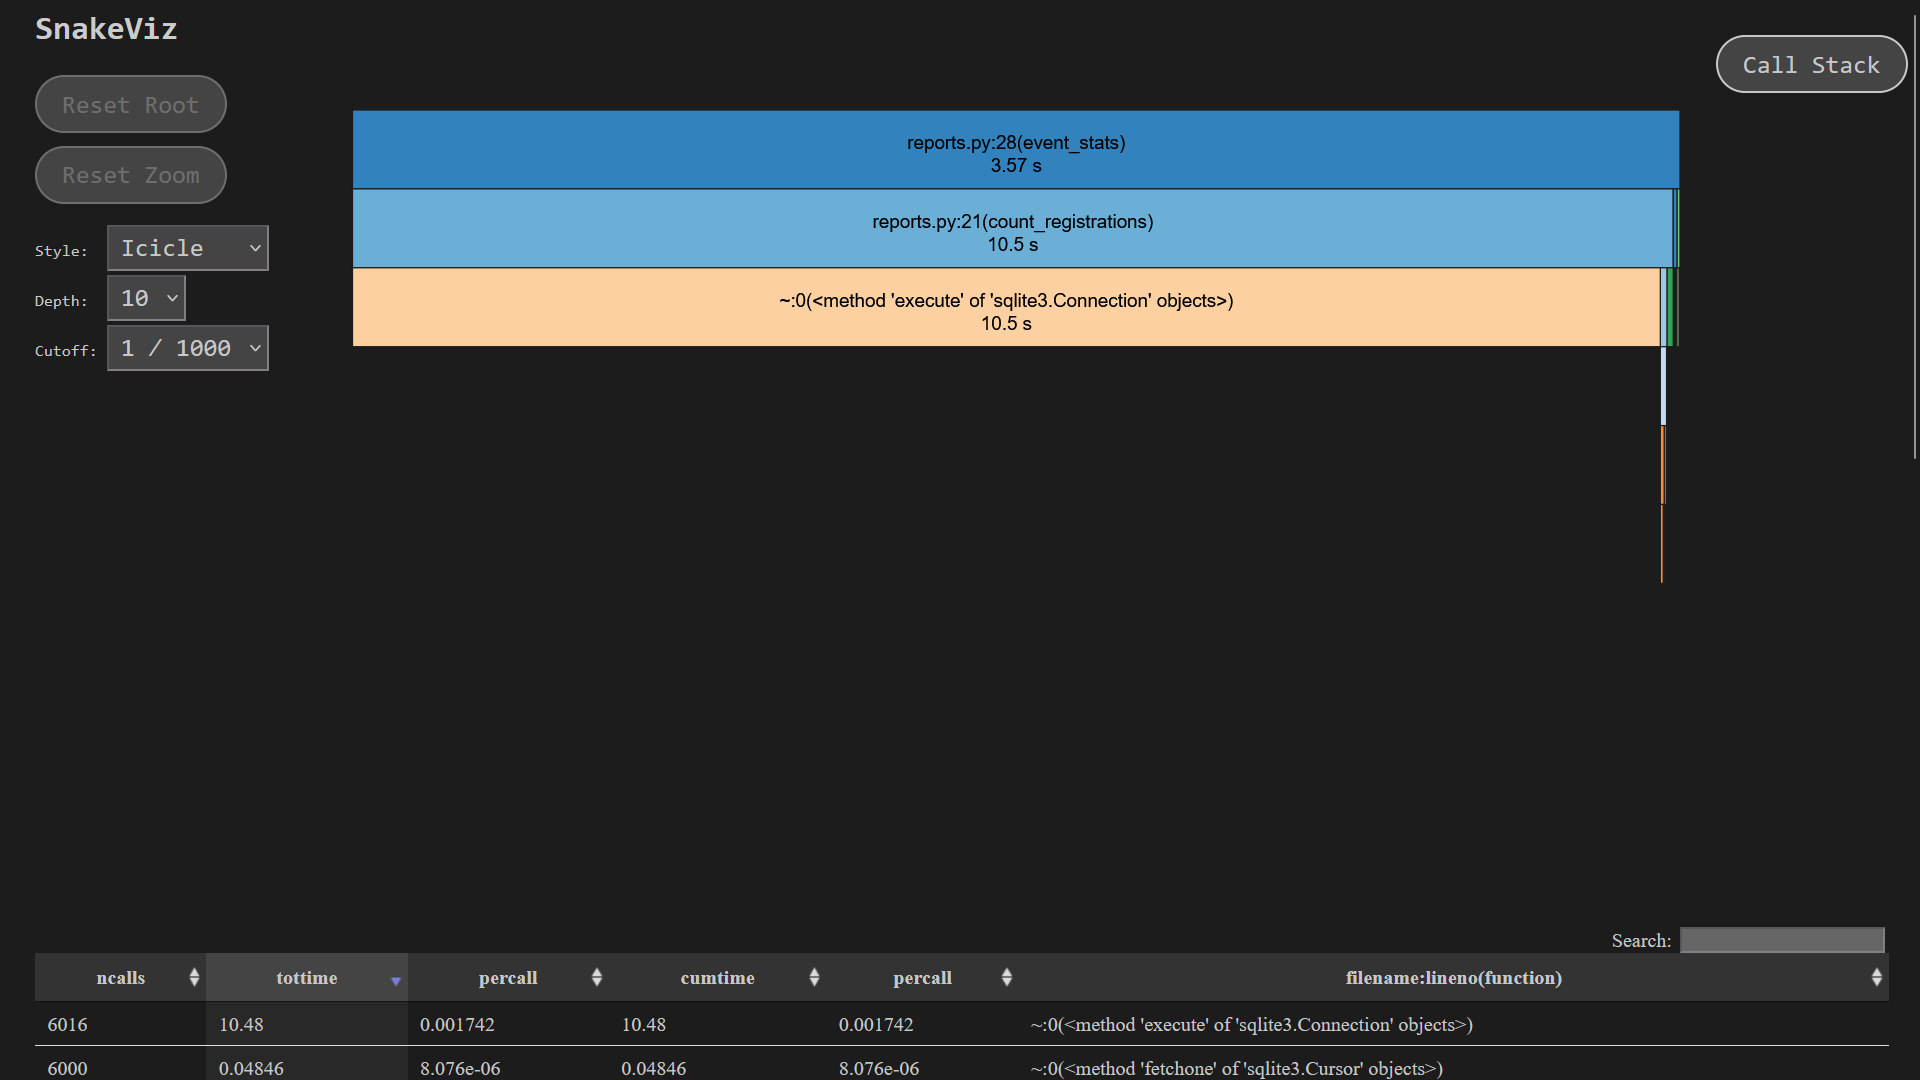
\includegraphics[width=\textwidth]{figures/before_snakeviz.png}\\[2pt]
      {\scriptsize SnakeViz, before}
    \end{column}
  \end{columns}
\end{frame}

% ---------------------------------------------------------------------
% 8: the key slide
\begin{frame}{Optimisation: before vs after}
  \begin{columns}[c]
    \begin{column}{0.52\textwidth}
      \small
      \textbf{Fix 1:} each report = \textbf{one} \code{LEFT JOIN} + \code{GROUP BY} query\\
      \textbf{Fix 2:} indexes on \code{registrations(event_id)}, \code{events(venue_id, start_time)}, \code{events(category)}
      \vspace{6pt}

      \footnotesize
      \begin{tabular}{@{}l r r r@{}}
        \toprule
        & \textbf{SQL calls} & \textbf{Before} & \textbf{After} \\
        \midrule
        Event stats  & 2001 $\rightarrow$ 1 & 3598 ms & 9.1 ms \\
        Categories   & 2001 $\rightarrow$ 1 & 3503 ms & 6.5 ms \\
        Venues       & 2011 $\rightarrow$ 1 & 3753 ms & 6.0 ms \\
        Search (3x)  & 3 $\rightarrow$ 3    & 63 ms   & 10.9 ms \\
        \midrule
        \textbf{Total} & \textbf{6016 $\rightarrow$ 6} & \textbf{10.9 s} & \textbf{32.6 ms} \\
        \bottomrule
      \end{tabular}

      \vspace{6pt}
      \small\textbf{About 335$\times$ faster}, same numbers (tests unchanged)
    \end{column}
    \begin{column}{0.46\textwidth}
      \centering
      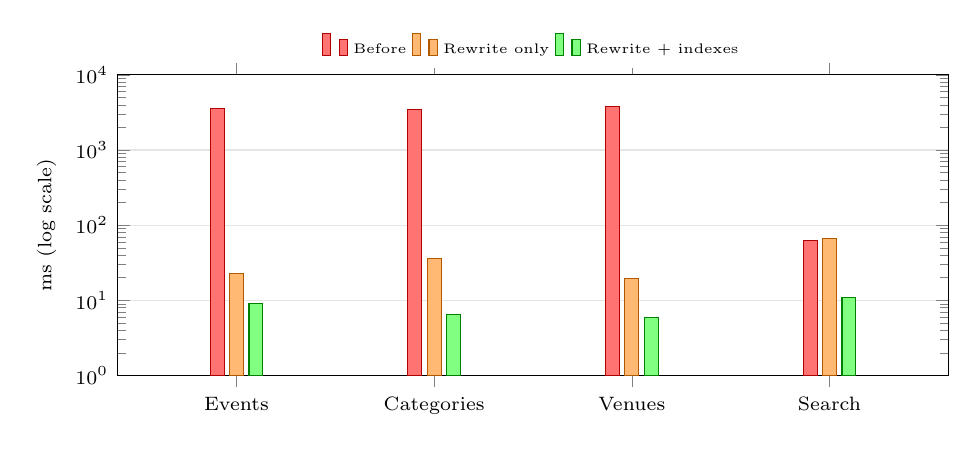
\begin{tikzpicture}
        \begin{axis}[
            ybar, ymode=log, log origin=infty,
            width=\textwidth, height=5.4cm,
            bar width=5pt, ymin=1, ymax=10000,
            ylabel={ms (log scale)}, ylabel style={font=\scriptsize},
            xtick={1,2,3,4}, xticklabels={Events, Categories, Venues, Search},
            tick label style={font=\scriptsize},
            enlarge x limits=0.2, ymajorgrids, grid style={black!10},
            legend style={at={(0.5,1.02)}, anchor=south, legend columns=3, draw=none, font=\tiny},
          ]
          \addplot[fill=red!55, draw=red!70!black]       coordinates {(1,3597.5) (2,3502.5) (3,3752.9) (4,63.1)};
          \addplot[fill=orange!55, draw=orange!70!black] coordinates {(1,22.9) (2,36.0) (3,19.8) (4,66.0)};
          \addplot[fill=green!50, draw=green!50!black]   coordinates {(1,9.1) (2,6.5) (3,6.0) (4,10.9)};
          \legend{Before, {Rewrite only}, {Rewrite + indexes}}
        \end{axis}
      \end{tikzpicture}
      {\scriptsize Query plan: \code{SCAN registrations} $\rightarrow$\\ \code{SEARCH ... USING COVERING INDEX idx_registrations_event}}
    \end{column}
  \end{columns}
\end{frame}

% ---------------------------------------------------------------------
% 9
\begin{frame}[fragile]{Git and Bash automation}
  \begin{columns}[T]
    \begin{column}{0.48\textwidth}
      \textbf{Git}
      \begin{itemize}\small
        \item Small commits, each leaving tests passing
        \item Convention: \code{feat:} \code{test:} \code{perf:} \code{chore:} \code{docs:}
        \item Naive version + baseline committed \emph{before} the fix, so the history shows what was measured
        \item \code{.gitattributes} keeps \code{.sh} files LF
      \end{itemize}
\begin{lstlisting}
perf: replace N+1 report loops with JOIN + GROUP BY queries
docs: record baseline profile of naive reports
feat: add admin reports page (naive N+1 version)
\end{lstlisting}
    \end{column}
    \begin{column}{0.48\textwidth}
      \textbf{Bash} (\code{set -euo pipefail})
      \begin{itemize}\small
        \item \code{setup.sh}: venv, install, DB, indexes, admin
        \item \code{run.sh}, \code{seed.sh [N]}, \code{test.sh}
        \item \code{profile.sh <label>}: separate DB, seed 2000 events, cProfile, query plans
        \item \code{build_docs.sh}: compile LaTeX
        \item Works in Git Bash on Windows: \code{venv/Scripts} vs \code{venv/bin}, \code{python -m flask}
      \end{itemize}
    \end{column}
  \end{columns}
\end{frame}

% ---------------------------------------------------------------------
% 10
\begin{frame}{Live demo}
  \begin{enumerate}
    \item \code{./scripts/setup.sh} then \code{./scripts/seed.sh}, then \code{./scripts/run.sh}
    \item Student: search \emph{workshop}, open an event, \textbf{Register}, then try again (rejected)
    \item My registrations, then \textbf{Cancel}
    \item Admin: new event at a busy venue and time, \textbf{clash rejected}
    \item Participants, then \textbf{Export CSV}
    \item Reports page
    \item \code{./scripts/test.sh}: 45 passed
  \end{enumerate}
  \vspace{6pt}
  \small Logins: \code{admin@campus.local / admin123} $\cdot$ \code{student1@campus.local / student123}
\end{frame}

% ---------------------------------------------------------------------
% 11
\begin{frame}
  \centering
  \vspace{1cm}
  {\Huge Thank you!}\\[0.8cm]
  {\Large Questions?}\\[1cm]
  \small Code, tests, profiling results: \code{README.md} $\cdot$ \code{profiling/RESULTS.md}\\[4pt]
  \footnotesize AI assistance declared --- see report Section 10 and \code{AI_USAGE.md}.
\end{frame}

\end{document}
